\documentclass[12pt]{article}
\usepackage[a4paper, margin=2cm]{geometry}
\usepackage{graphicx}
\usepackage{tikz}
\usetikzlibrary{arrows.meta, shapes, positioning, patterns}
\usepackage{pgfplots}
\pgfplotsset{compat=1.18}

\title{Images and TikZ Diagrams Test}
\author{TeX Live API}
\date{\today}

\begin{document}
\maketitle

\section{TikZ: Force Diagram}

\begin{figure}[htbp]
\centering
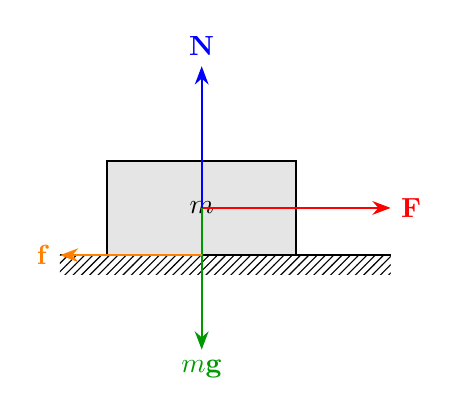
\begin{tikzpicture}[scale=1.2, >=Stealth]
  % Block
  \draw[thick, fill=gray!20] (0,0) rectangle (2,1);
  \node at (1, 0.5) {$m$};
  % Ground
  \draw[thick] (-0.5,0) -- (3,0);
  \fill[pattern=north east lines] (-0.5,-0.2) rectangle (3,0);
  % Forces
  \draw[->, thick, red]   (1,0.5) -- (3,0.5) node[right]{$\mathbf{F}$};
  \draw[->, thick, blue]  (1,0.5) -- (1,2)   node[above]{$\mathbf{N}$};
  \draw[->, thick, green!60!black] (1,0.5) -- (1,-1) node[below]{$m\mathbf{g}$};
  \draw[->, thick, orange](1,0)   -- (-0.5,0) node[left]{$\mathbf{f}$};
\end{tikzpicture}
\caption{Free body diagram showing applied force $\mathbf{F}$, normal force $\mathbf{N}$,
  weight $m\mathbf{g}$, and friction $\mathbf{f}$.}
\end{figure}

\section{pgfplots: Function Plots}

\begin{figure}[htbp]
\centering
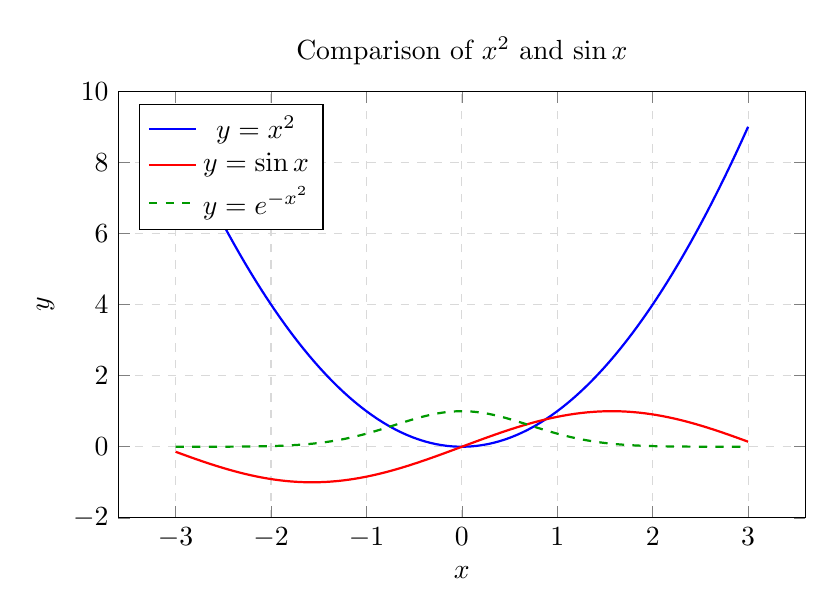
\begin{tikzpicture}
\begin{axis}[
  xlabel={$x$}, ylabel={$y$},
  grid=major, grid style={dashed, gray!30},
  width=0.85\textwidth, height=7cm,
  legend pos=north west,
  title={Comparison of $x^2$ and $\sin x$},
]
  \addplot[blue, thick, domain=-3:3, samples=100] {x^2};
  \addlegendentry{$y = x^2$}
  \addplot[red, thick, domain=-3:3, samples=100] {sin(deg(x))};
  \addlegendentry{$y = \sin x$}
  \addplot[green!60!black, thick, dashed, domain=-3:3, samples=100] {exp(-x^2)};
  \addlegendentry{$y = e^{-x^2}$}
\end{axis}
\end{tikzpicture}
\caption{Function plots generated with pgfplots.}
\end{figure}

\section{TikZ: Circuit (Conceptual)}

\begin{figure}[htbp]
\centering
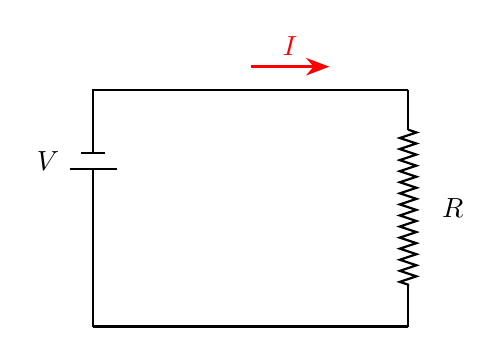
\begin{tikzpicture}[>=Stealth, thick]
  % Battery
  \draw (0,0) -- (0,2);
  \draw (-0.3,2) -- (0.3,2);
  \draw (-0.15,2.2) -- (0.15,2.2);
  \node[left] at (-0.3, 2.1) {$V$};
  % Wires
  \draw (0,2.2) -- (0,3) -- (4,3);
  \draw (0,0) -- (4,0);
  % Resistor (zigzag)
  \draw (4,3) -- (4,2.5);
  \draw[decorate, decoration={zigzag, segment length=4, amplitude=3}] (4,2.5) -- (4,0.5);
  \draw (4,0.5) -- (4,0);
  \node[right] at (4.3, 1.5) {$R$};
  % Current arrow
  \draw[->, red, very thick] (2,3.3) -- (3,3.3) node[midway, above] {$I$};
\end{tikzpicture}
\caption{Simple circuit with battery and resistor.}
\end{figure}

\end{document}
